
\section{Results and Discussion}

\begin{table}
  \caption{Evaluation of End-to-end error correction on Thai social data on various systems}
  \begin{tabular}{lcc}
    \toprule
    Model & Type & GLEU \\
    \midrule
    Do nothing & - & 0.8845 \\
    Oracle & - & 1.0000 \\
    \midrule
    \textbf{Off the shelf} & \\
    Hunspell & 2-Stage & 0.8267 \\
    PyThaiNLP & 2-Stage & 0.8612 \\
    \midrule
    \textbf{Trained} & \\
    BiGRU & End-to-End & 0.5486 \\
    % Copy-Augmented Transformer (not tuned)  & End-to-End & 0.6914 \\
    Copy-Augmented Transformer & End-to-End & 0.7581 \\
    Hunspell & 2-Stage & 0.8598 \\
    \midrule
    Ours & 2-Stage & 0.9274 \\
    Ours (SentencePiece) & 2-Stage & 0.9326 \\
    % Ours (SentencePiece + Tuned Detection) & 2-Stage & 0.9329 \\
    Ours (Oracle Detection) & 2-Stage & 0.9490 \\
    Ours (SentencePiece + Oracle Detection) & 2-Stage & 0.9533 \\
    \bottomrule
  \end{tabular}
  \label{tab:e2e_ugwc}
\end{table}

Our approach was evaluated on two tasks: error correction on our Thai UGWC dataset, and error correction on the English Conll 2014 GEC task. With the Conll 2014 GEC task chosen for its ease of access to other researchers as the Thai UGWC dataset is not publicly available.

\subsection{Thai UGWC}

The results on the Thai UGWC are shown in Table~\ref{tab:e2e_ugwc}.
[investigate hunspell]
Our proposed method outperform all existing solutions on the UGWC task. Interestingly, by grouping methods into 2-stage error correction (i.e. PyThaiNLP, Hunspell, and Ours) and end-to-end correction (i.e. Bi-GRU, and Copy-Augmented) we can see a clear trend that 2-stage methods performs significantly better on the Thai UGWC task. Error analysis shows that the end-to-end systems have trouble processing longer lines due to its eagerness to perform correction where none is required. [need example] [need to investigate for more reasons]

\begin{figure}
  \centering
  \newlength{\plotwidth}
  \setlength{\plotwidth}{0.7\textwidth}
  % \begin{subfigure}[b]{0.48\textwidth}
      \centering
      % \includegraphics[width=\textwidth]{Graph2}
      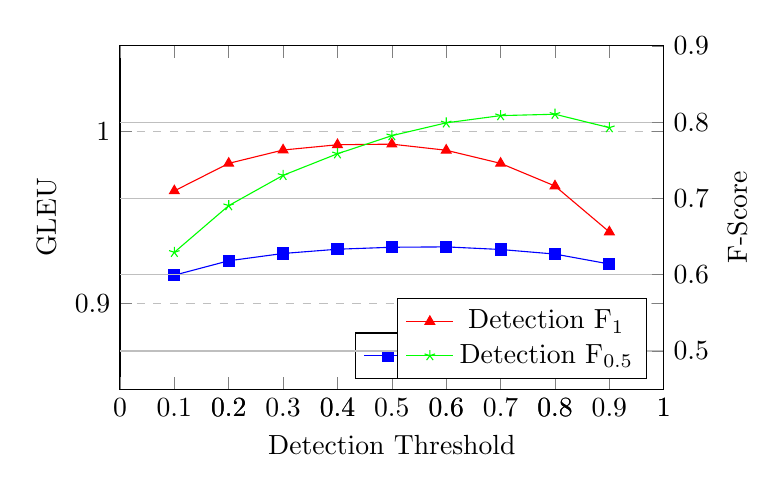
\begin{tikzpicture}
      \pgfplotsset{width=7cm,compat=1.3}
      \begin{axis}[
          xlabel={Detection Threshold},
          ylabel={GLEU},
          xmin=0, xmax=1.0,
          ymin=0.85, ymax=1.05,
          width=\plotwidth,
          height=0.7\plotwidth,
          xtick={0.1,0.2,0.3,0.4,0.5,0.6,0.7,0.8,0.9,1},
          ytick={0.1,0.2,0.3,0.4,0.5,0.6,0.7,0.8,0.9,1},
          legend pos=south east,
          ymajorgrids=true,
          grid style=dashed,
      ]

      \addplot[
          color=blue,
          mark=square*,
          ]
          coordinates {
            (0.1, 0.916363)
            (0.2, 0.924753)
            (0.3, 0.92901)
            (0.4, 0.931486)
            (0.5, 0.932635)
            (0.6, 0.932851)
            (0.7, 0.931332)
            (0.8, 0.928659)
            (0.9, 0.922877)
          };
      \legend{Correction GLEU}
      \end{axis}
      
      \begin{axis}[
          axis y line*=right,
          ylabel={F-Score},
          xmin=0, xmax=1.0,
          ymin=0.45, ymax=0.90,
          width=\plotwidth,
          height=0.7\plotwidth,
          ytick={0.1,0.2,0.3,0.4,0.5,0.6,0.7,0.8,0.9,1},
          legend pos=south east,
          ymajorgrids=true,
      ]
      \addplot[
          color=red,
          mark=triangle*,
          ]
          coordinates {
            (0.1, 0.7098)
            (0.2, 0.7459)
            (0.3, 0.7634)
            (0.4, 0.7703)
            (0.5, 0.7711)
            (0.6, 0.7631)
            (0.7, 0.7459)
            (0.8, 0.7162)
            (0.9, 0.6560)
          };
      \addplot[
          color=green,
          mark=star,
          ]
          coordinates {
            (0.1, 0.6293)
            (0.2, 0.6905)
            (0.3, 0.7302)
            (0.4, 0.7585)
            (0.5, 0.7822)
            (0.6, 0.7990)
            (0.7, 0.8085)
            (0.8, 0.8103)
            (0.9, 0.7927)
          };
      \legend{Detection F\textsubscript{1}, Detection F\textsubscript{0.5}}
      \end{axis}
      \end{tikzpicture}
      \caption{Evaluation of our error correction at varying detection sensitivity.}
      \label{fig:detect_threshold}
  % \Description{The performance of the supervised and CVT model as percent of training set is varied.}
\end{figure}

\begin{table}
  \caption{Evaluation of End-to-end error correction with SentencePiece as the unit token on Thai social data on varying detection sensitivity}
  \label{tab:e2e_detect_sense}
  \begin{tabular}{lccccc}
    \toprule
    Detection Threshold & GLEU & $f_{0.5}$ & $f_1$ & precision & recall \\
    \midrule
    0.1 & 0.9164 & 0.6293 & 0.7098 & 0.5851 & 0.9021 \\
    0.2 & 0.9248 & 0.6905 & 0.7459 & 0.6579 & 0.8611 \\
    0.3 & 0.9290 & 0.7302 & 0.7634 & 0.7097 & 0.8258 \\
    0.4 & 0.9315 & 0.7585 & 0.7703 & 0.7508 & 0.7909 \\
    0.5 & 0.9326 & 0.7822 & \textbf{0.7711} & 0.7899 & 0.7532 \\
    0.6 & \textbf{0.9329} & 0.7990 & 0.7631 & 0.8248 & 0.7100 \\
    0.7 & 0.9313 & 0.8085 & 0.7459 & 0.8564 & 0.6607 \\
0.8 & 0.9287 & \textbf{0.8103} & 0.7162 & 0.8881 & 0.6001 \\
    0.9 & 0.9229 & 0.7927 & 0.6560 & 0.9206 & 0.5095 \\
    \bottomrule
\end{tabular}
\end{table}

\begin{figure}
    \centering
    \label{fig:thresholding_prediction}
    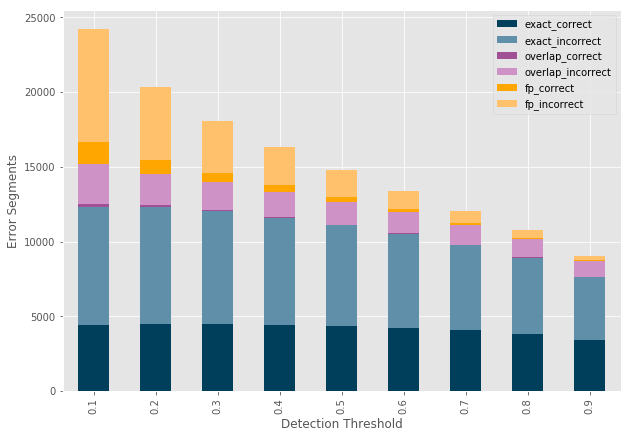
\includegraphics[width=12.5cm]{diagrams/thresholding-prediction.png}
    \caption{Visualization of corrections performed by our system at varying detection sensitivity on the Thai UGWC test-set. The y-axis represent the number of altered segments of text by our system. Each of the segment is the results of the detection stage, and the correction stage. The detection can either be an exact detection of the actual error, a partial overlap with the actual error, or a false positive detection. Corrections made to the error segment can either produce a correct or an incorrect resulting text. Correct alteration of the text with either an exact detection (dark blue) or a overlapping detection (dark purple) results in the errors in the text being corrected. Incorrect alteration from false positive (light orange) detection results in errors being introduced to the text. While it is inconclusive to determine if the incorrect alteration of the text with either an exact detection (light blue) or a overlapping detection (light purple) will yeild a better or worse resulting text.}
\end{figure}

\subsection*{Detection Sensitivity}
Evaluation of our proposed method at varying detection sensitivity are shown in Fig~\ref{fig:detect_threshold} and Table~\ref{tab:e2e_detect_sense}. Results show a stronger correlation between the $F_1$ detection score and end-to-end GLEU score than that of $F_{0.5}$ detection score. This is non-intuitive as error correction metrics such as M2 uses the $F_{0.5}$ to favor precision over recall [REF]. However, further investigation shows that the deterioration in performance is a result of reducted number of exact detection, where the detector is able to identify the exact boundaries of the erroneous text which leads to an increased number of error segments being uncorrectable by the correction stage [Need to ref some example].

\begin{table}
  \caption{Evaluation of End-to-end error correction on the GEC Conll-2014 on various systems}
  \label{tab:e2e_conll_all}
  \begin{tabular}{lcccc}
    \toprule
    Model & M2 & GLEU \\
    \midrule
    Do nothing & 0.0000 & 0.5663 \\
    Oracle & 1.0000 & 0.8187 \\
    \midrule
    \textbf{Literature} & \\
    \textbf{BiGRU} & \textbf{0.4276} & - \\
    SMT + BiGRU & 0.5625 & - \\
    Copy-Augmented Transformer & 0.5642	& - \\
    Copy-Augmented Transformer + (Pre-trained) & 0.6115 & - \\
    \midrule
    \textbf{Reproduced} & \\
    BiGRU without Lang 8 & 0.2158 & 0.5354 \\
    \textbf{BiGRU} & \textbf{0.4288} & 0.5931 \\
    \midrule
    \textbf{Ours} & 0.0195 & 0.5630 \\
    \bottomrule
\end{tabular}
\end{table}


\begin{table}
\caption{Evaluation of End-to-end error correction on the misspelling subset of GEC Conll-2014 on various systems}
  \label{tab:e2e_conll_misspell}
  \begin{tabular}{lccccccc}
    \toprule
    & \multicolumn{3}{c}{Original} & \multicolumn{4}{c}{Repacked}\\
    Model & Precision & Recall & M2 & Precision & Recall & M2 & GLEU\\
    \midrule
    Pre-corrected & \textbf{0.9913} & 0.9048 & \textbf{0.9727} & 0.0000 & 0.0000 & 0.0000 & 0.7520 \\
    Oracle & 0.9917 & 0.9896 & 0.9900 & 0.9826 & 0.9912 & 0.9843 & 0.7767 \\
    \midrule
    BiGRU & 0.8163 & 0.8280 & 0.8186 & 0.0205 & 0.0395 & 0.0227 & 0.6812 \\
    BiGRU + Lang8 & 0.9307 & 0.8661 & 0.9170 & 0.1449 & \textbf{0.1360} & 0.1430 & 0.7376 \\
    \midrule
    Ours & 0.9557 & \textbf{0.9082} & 0.9458 & \textbf{0.1792} & 0.0833 & \textbf{0.1457} & \textbf{0.7540} \\
    Ours + Oracle Detection & 0.9712 & 0.9183 & 0.9601 & 0.4250 & 0.1491 & 0.3102 & 0.7606 \\
    \bottomrule
\end{tabular}
\end{table}

\subsection{English GEC Conll-2014}

Our method was evaluated on both the full grammatical error correction (GEC) task and subsetting the Conll-2014 for measuring only misspelling corrections. The results are shown in Table~\ref{tab:e2e_conll_all} and Table~\ref{tab:e2e_conll_misspell}.

Our method unsurprisingly performs very poorly on the GEC task. Although the GLEU may high but score itself is still lower than doing nothing.

Evaluating our model on the misspelling subset of the Conll-2014 shows a different story. Our model is able to perform compeitivly when compared to the BiGRU model on both M2 and GLEU score on the repacked testset. While the original M2 testset is not comparible as the majority of the corrections scored is from the pre-correction rather than the correction applied by the systems. This results in both of the systems scoring lower that the precorrected input as score detection from false-positive are over weighted by M2.
